\documentclass[1p]{elsarticle_modified}
%\bibliographystyle{elsarticle-num}

%\usepackage[colorlinks]{hyperref}
%\usepackage{abbrmath_seonhwa} %\Abb, \Ascr, \Acal ,\Abf, \Afrak
\usepackage{amsfonts}
\usepackage{amssymb}
\usepackage{amsmath}
\usepackage{amsthm}
\usepackage{scalefnt}
\usepackage{amsbsy}
\usepackage{kotex}
\usepackage{caption}
\usepackage{subfig}
\usepackage{color}
\usepackage{graphicx}
\usepackage{xcolor} %% white, black, red, green, blue, cyan, magenta, yellow
\usepackage{float}
\usepackage{setspace}
\usepackage{hyperref}

\usepackage{tikz}
\usetikzlibrary{arrows}

\usepackage{multirow}
\usepackage{array} % fixed length table
\usepackage{hhline}

%%%%%%%%%%%%%%%%%%%%%
\makeatletter
\renewcommand*\env@matrix[1][\arraystretch]{%
	\edef\arraystretch{#1}%
	\hskip -\arraycolsep
	\let\@ifnextchar\new@ifnextchar
	\array{*\c@MaxMatrixCols c}}
\makeatother %https://tex.stackexchange.com/questions/14071/how-can-i-increase-the-line-spacing-in-a-matrix
%%%%%%%%%%%%%%%

\usepackage[normalem]{ulem}

\newcommand{\msout}[1]{\ifmmode\text{\sout{\ensuremath{#1}}}\else\sout{#1}\fi}
%SOURCE: \msout is \stkout macro in https://tex.stackexchange.com/questions/20609/strikeout-in-math-mode

\newcommand{\cancel}[1]{
	\ifmmode
	{\color{red}\msout{#1}}
	\else
	{\color{red}\sout{#1}}
	\fi
}

\newcommand{\add}[1]{
	{\color{blue}\uwave{#1}}
}

\newcommand{\replace}[2]{
	\ifmmode
	{\color{red}\msout{#1}}{\color{blue}\uwave{#2}}
	\else
	{\color{red}\sout{#1}}{\color{blue}\uwave{#2}}
	\fi
}

\newcommand{\Sol}{\mathcal{S}} %segment
\newcommand{\D}{D} %diagram
\newcommand{\A}{\mathcal{A}} %arc


%%%%%%%%%%%%%%%%%%%%%%%%%%%%%5 test

\def\sl{\operatorname{\textup{SL}}(2,\Cbb)}
\def\psl{\operatorname{\textup{PSL}}(2,\Cbb)}
\def\quan{\mkern 1mu \triangleright \mkern 1mu}

\theoremstyle{definition}
\newtheorem{thm}{Theorem}[section]
\newtheorem{prop}[thm]{Proposition}
\newtheorem{lem}[thm]{Lemma}
\newtheorem{ques}[thm]{Question}
\newtheorem{cor}[thm]{Corollary}
\newtheorem{defn}[thm]{Definition}
\newtheorem{exam}[thm]{Example}
\newtheorem{rmk}[thm]{Remark}
\newtheorem{alg}[thm]{Algorithm}

\newcommand{\I}{\sqrt{-1}}
\begin{document}

%\begin{frontmatter}
%
%\title{Boundary parabolic representations of knots up to 8 crossings}
%
%%% Group authors per affiliation:
%\author{Yunhi Cho} 
%\address{Department of Mathematics, University of Seoul, Seoul, Korea}
%\ead{yhcho@uos.ac.kr}
%
%
%\author{Seonhwa Kim} %\fnref{s_kim}}
%\address{Center for Geometry and Physics, Institute for Basic Science, Pohang, 37673, Korea}
%\ead{ryeona17@ibs.re.kr}
%
%\author{Hyuk Kim}
%\address{Department of Mathematical Sciences, Seoul National University, Seoul 08826, Korea}
%\ead{hyukkim@snu.ac.kr}
%
%\author{Seokbeom Yoon}
%\address{Department of Mathematical Sciences, Seoul National University, Seoul, 08826,  Korea}
%\ead{sbyoon15@snu.ac.kr}
%
%\begin{abstract}
%We find all boundary parabolic representation of knots up to 8 crossings.
%
%\end{abstract}
%\begin{keyword}
%    \MSC[2010] 57M25 
%\end{keyword}
%
%\end{frontmatter}

%\linenumbers
%\tableofcontents
%
\newcommand\colored[1]{\textcolor{white}{\rule[-0.35ex]{0.8em}{1.4ex}}\kern-0.8em\color{red} #1}%
%\newcommand\colored[1]{\textcolor{white}{ #1}\kern-2.17ex	\textcolor{white}{ #1}\kern-1.81ex	\textcolor{white}{ #1}\kern-2.15ex\color{red}#1	}

{\Large $\underline{12a_{1145}~(K12a_{1145})}$}

\setlength{\tabcolsep}{10pt}
\renewcommand{\arraystretch}{1.6}
\vspace{1cm}\begin{tabular}{m{100pt}>{\centering\arraybackslash}m{274pt}}
\multirow{5}{120pt}{
	\centering
	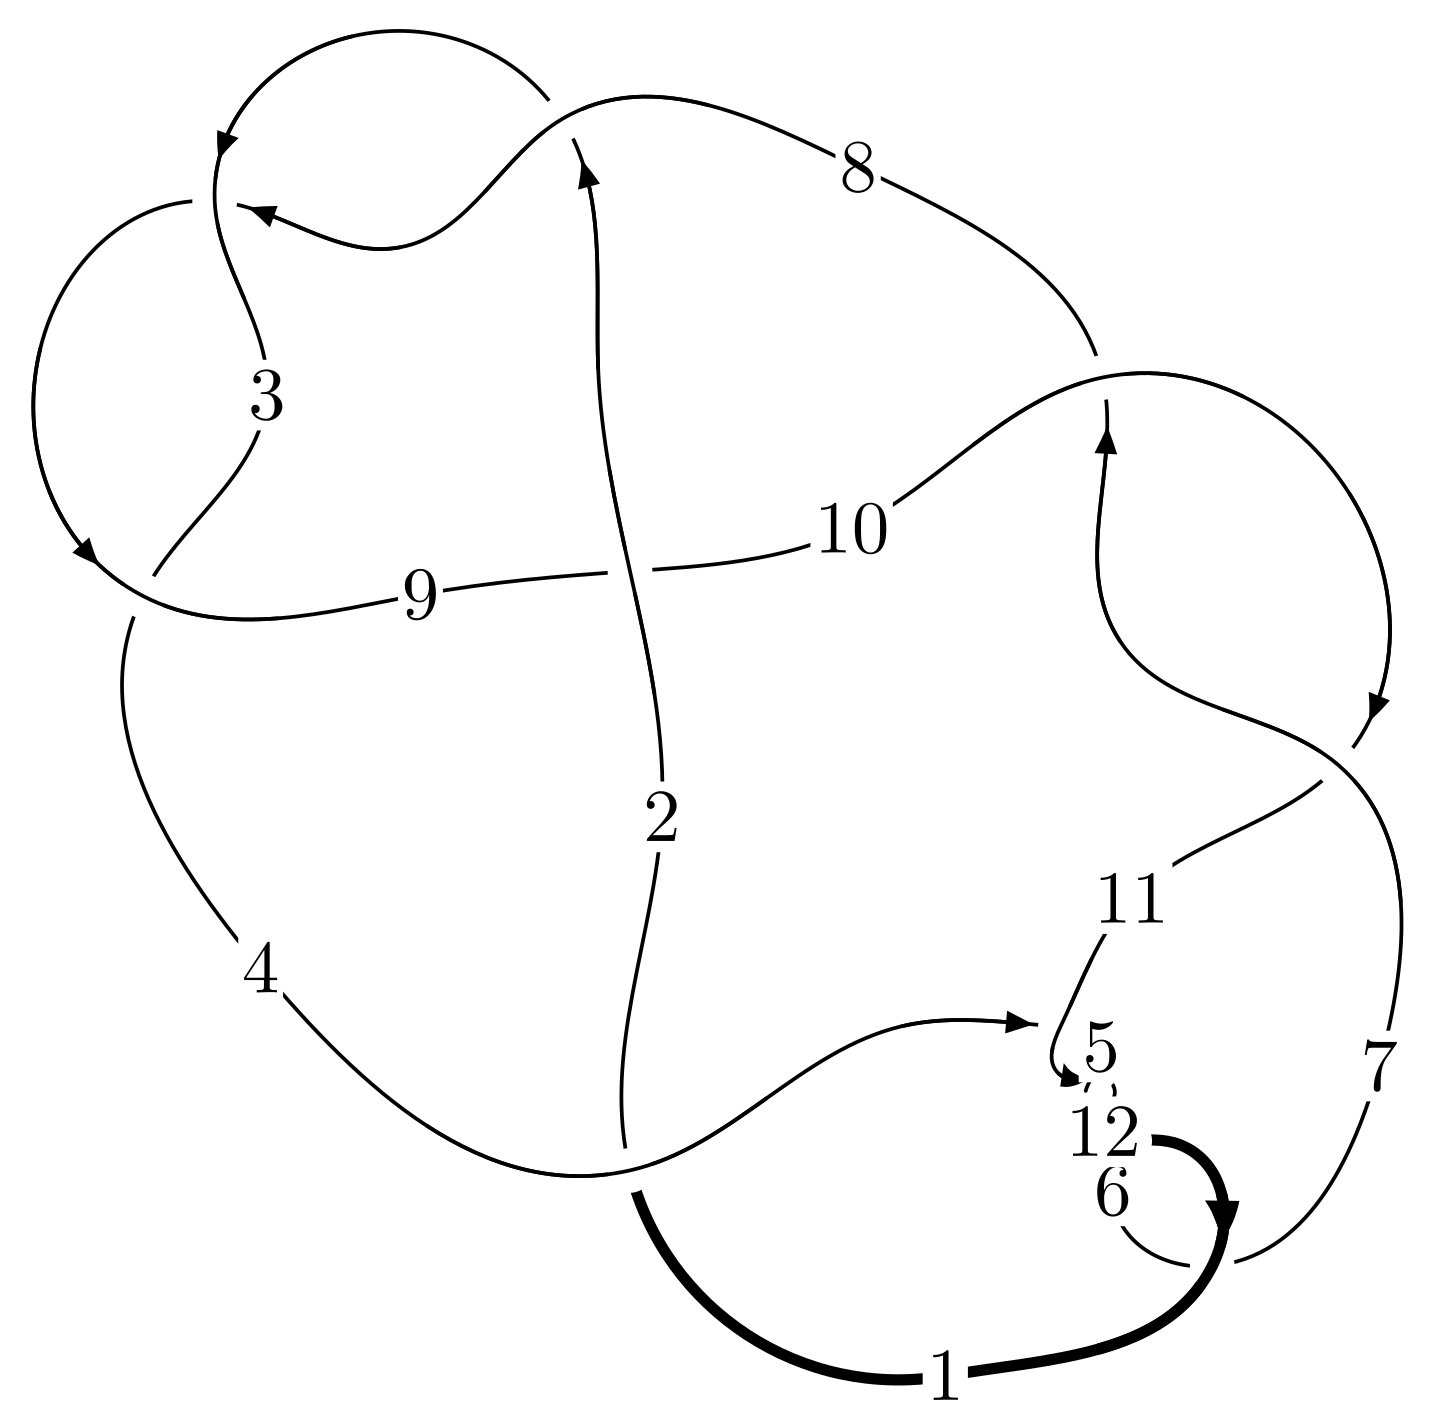
\includegraphics[width=112pt]{../../../GIT/diagram.site/Diagrams/png/1946_12a_1145.png}\\
\ \ \ A knot diagram\footnotemark}&
\allowdisplaybreaks
\textbf{Linearized knot diagam} \\
\cline{2-2}
 &
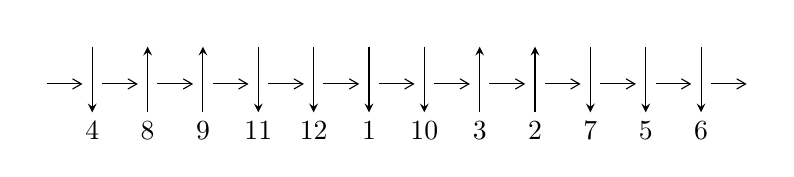
\begin{tikzpicture}[x=20pt, y=17pt]
	% nodes
	\node (C0) at (0, 0) {};
	\node (C1) at (1, 0) {};
	\node (C1U) at (1, +1) {};
	\node (C1D) at (1, -1) {4};

	\node (C2) at (2, 0) {};
	\node (C2U) at (2, +1) {};
	\node (C2D) at (2, -1) {8};

	\node (C3) at (3, 0) {};
	\node (C3U) at (3, +1) {};
	\node (C3D) at (3, -1) {9};

	\node (C4) at (4, 0) {};
	\node (C4U) at (4, +1) {};
	\node (C4D) at (4, -1) {11};

	\node (C5) at (5, 0) {};
	\node (C5U) at (5, +1) {};
	\node (C5D) at (5, -1) {12};

	\node (C6) at (6, 0) {};
	\node (C6U) at (6, +1) {};
	\node (C6D) at (6, -1) {1};

	\node (C7) at (7, 0) {};
	\node (C7U) at (7, +1) {};
	\node (C7D) at (7, -1) {10};

	\node (C8) at (8, 0) {};
	\node (C8U) at (8, +1) {};
	\node (C8D) at (8, -1) {3};

	\node (C9) at (9, 0) {};
	\node (C9U) at (9, +1) {};
	\node (C9D) at (9, -1) {2};

	\node (C10) at (10, 0) {};
	\node (C10U) at (10, +1) {};
	\node (C10D) at (10, -1) {7};

	\node (C11) at (11, 0) {};
	\node (C11U) at (11, +1) {};
	\node (C11D) at (11, -1) {5};

	\node (C12) at (12, 0) {};
	\node (C12U) at (12, +1) {};
	\node (C12D) at (12, -1) {6};
	\node (C13) at (13, 0) {};

	% arrows
	\draw[->,>={angle 60}]
	(C0) edge (C1) (C1) edge (C2) (C2) edge (C3) (C3) edge (C4) (C4) edge (C5) (C5) edge (C6) (C6) edge (C7) (C7) edge (C8) (C8) edge (C9) (C9) edge (C10) (C10) edge (C11) (C11) edge (C12) (C12) edge (C13) ;	\draw[->,>=stealth]
	(C1U) edge (C1D) (C2D) edge (C2U) (C3D) edge (C3U) (C4U) edge (C4D) (C5U) edge (C5D) (C6U) edge (C6D) (C7U) edge (C7D) (C8D) edge (C8U) (C9D) edge (C9U) (C10U) edge (C10D) (C11U) edge (C11D) (C12U) edge (C12D) ;
	\end{tikzpicture} \\
\hhline{~~} \\& 
\textbf{Solving Sequence} \\ \cline{2-2} 
 &
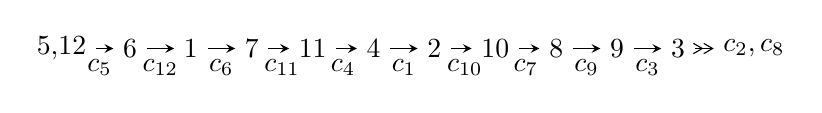
\begin{tikzpicture}[x=22pt, y=7pt]
	% node
	\node (A0) at (-1/8, 0) {5,12};
	\node (A1) at (1, 0) {6};
	\node (A2) at (2, 0) {1};
	\node (A3) at (3, 0) {7};
	\node (A4) at (4, 0) {11};
	\node (A5) at (5, 0) {4};
	\node (A6) at (6, 0) {2};
	\node (A7) at (7, 0) {10};
	\node (A8) at (8, 0) {8};
	\node (A9) at (9, 0) {9};
	\node (A10) at (10, 0) {3};
	\node (C1) at (1/2, -1) {$c_{5}$};
	\node (C2) at (3/2, -1) {$c_{12}$};
	\node (C3) at (5/2, -1) {$c_{6}$};
	\node (C4) at (7/2, -1) {$c_{11}$};
	\node (C5) at (9/2, -1) {$c_{4}$};
	\node (C6) at (11/2, -1) {$c_{1}$};
	\node (C7) at (13/2, -1) {$c_{10}$};
	\node (C8) at (15/2, -1) {$c_{7}$};
	\node (C9) at (17/2, -1) {$c_{9}$};
	\node (C10) at (19/2, -1) {$c_{3}$};
	\node (A11) at (45/4, 0) {$c_{2},c_{8}$};

	% edge
	\draw[->,>=stealth]	
	(A0) edge (A1) (A1) edge (A2) (A2) edge (A3) (A3) edge (A4) (A4) edge (A5) (A5) edge (A6) (A6) edge (A7) (A7) edge (A8) (A8) edge (A9) (A9) edge (A10) ;
	\draw[->>,>={angle 60}]	
	(A10) edge (A11);
\end{tikzpicture} \\ 

\end{tabular} \\

\footnotetext{
The image of knot diagram is generated by the software ``\textbf{Draw programme}" developed by Andrew Bartholomew(\url{http://www.layer8.co.uk/maths/draw/index.htm\#Running-draw}), where we modified some parts for our purpose(\url{https://github.com/CATsTAILs/LinksPainter}).
}\phantom \\ \newline 
\centering \textbf{Ideals for irreducible components\footnotemark of $X_{\text{par}}$} 
 
\begin{align*}
I^u_{1}&=\langle 
u^{39}- u^{38}+\cdots+2 u^2+1\rangle \\
\\
\end{align*}
\raggedright * 1 irreducible components of $\dim_{\mathbb{C}}=0$, with total 39 representations.\\
\footnotetext{All coefficients of polynomials are rational numbers. But the coefficients are sometimes approximated in decimal forms when there is not enough margin.}
\newpage
\renewcommand{\arraystretch}{1}
\centering \section*{I. $I^u_{1}= \langle u^{39}- u^{38}+\cdots+2 u^2+1 \rangle$}
\flushleft \textbf{(i) Arc colorings}\\
\begin{tabular}{m{7pt} m{180pt} m{7pt} m{180pt} }
\flushright $a_{5}=$&$\begin{pmatrix}1\\0\end{pmatrix}$ \\
\flushright $a_{12}=$&$\begin{pmatrix}0\\u\end{pmatrix}$ \\
\flushright $a_{6}=$&$\begin{pmatrix}1\\u^2\end{pmatrix}$ \\
\flushright $a_{1}=$&$\begin{pmatrix}- u\\- u^3+u\end{pmatrix}$ \\
\flushright $a_{7}=$&$\begin{pmatrix}- u^2+1\\- u^4+2 u^2\end{pmatrix}$ \\
\flushright $a_{11}=$&$\begin{pmatrix}u\\u\end{pmatrix}$ \\
\flushright $a_{4}=$&$\begin{pmatrix}- u^2+1\\- u^2\end{pmatrix}$ \\
\flushright $a_{2}=$&$\begin{pmatrix}u^7-4 u^5+4 u^3-2 u\\u^7-3 u^5+u\end{pmatrix}$ \\
\flushright $a_{10}=$&$\begin{pmatrix}- u^7+4 u^5-4 u^3+2 u\\- u^9+5 u^7-7 u^5+2 u^3+u\end{pmatrix}$ \\
\flushright $a_{8}=$&$\begin{pmatrix}- u^{12}+7 u^{10}-17 u^8+18 u^6-10 u^4+u^2+1\\- u^{14}+8 u^{12}-23 u^{10}+28 u^8-12 u^6-2 u^4+3 u^2\end{pmatrix}$ \\
\flushright $a_{9}=$&$\begin{pmatrix}u^{23}-14 u^{21}+\cdots-12 u^3+2 u\\u^{23}-13 u^{21}+\cdots+6 u^3+u\end{pmatrix}$ \\
\flushright $a_{3}=$&$\begin{pmatrix}- u^{33}+20 u^{31}+\cdots+12 u^3- u\\- u^{35}+21 u^{33}+\cdots+3 u^3+u\end{pmatrix}$\\&\end{tabular}
\flushleft \textbf{(ii) Obstruction class $= -1$}\\~\\
\flushleft \textbf{(iii) Cusp Shapes $= -4 u^{35}+88 u^{33}-864 u^{31}+4 u^{30}+4992 u^{29}-76 u^{28}-18852 u^{27}+632 u^{26}+48892 u^{25}-3020 u^{24}-89008 u^{23}+9160 u^{22}+113828 u^{21}-18396 u^{20}-99164 u^{19}+24724 u^{18}+52076 u^{17}-21696 u^{16}-6724 u^{15}+11000 u^{14}-12088 u^{13}-1160 u^{12}+9184 u^{11}-2344 u^{10}-2088 u^9+1456 u^8-600 u^7-192 u^6+400 u^5-112 u^4-36 u^3+32 u^2-8 u-2$}\\~\\
\newpage\renewcommand{\arraystretch}{1}
\flushleft \textbf{(iv) u-Polynomials at the component}\newline \\
\begin{tabular}{m{50pt}|m{274pt}}
Crossings & \hspace{64pt}u-Polynomials at each crossing \\
\hline $$\begin{aligned}c_{1},c_{7},c_{10}\end{aligned}$$&$\begin{aligned}
&u^{39}-5 u^{38}+\cdots+8 u+1
\end{aligned}$\\
\hline $$\begin{aligned}c_{2},c_{3},c_{8}\end{aligned}$$&$\begin{aligned}
&u^{39}- u^{38}+\cdots+2 u^2+1
\end{aligned}$\\
\hline $$\begin{aligned}c_{4},c_{5},c_{6}\\c_{11},c_{12}\end{aligned}$$&$\begin{aligned}
&u^{39}- u^{38}+\cdots+2 u^2+1
\end{aligned}$\\
\hline $$\begin{aligned}c_{9}\end{aligned}$$&$\begin{aligned}
&u^{39}+3 u^{38}+\cdots-64 u-11
\end{aligned}$\\
\hline
\end{tabular}\\~\\
\newpage\renewcommand{\arraystretch}{1}
\flushleft \textbf{(v) Riley Polynomials at the component}\newline \\
\begin{tabular}{m{50pt}|m{274pt}}
Crossings & \hspace{64pt}Riley Polynomials at each crossing \\
\hline $$\begin{aligned}c_{1},c_{7},c_{10}\end{aligned}$$&$\begin{aligned}
&y^{39}+39 y^{38}+\cdots+244 y-1
\end{aligned}$\\
\hline $$\begin{aligned}c_{2},c_{3},c_{8}\end{aligned}$$&$\begin{aligned}
&y^{39}-37 y^{38}+\cdots-4 y-1
\end{aligned}$\\
\hline $$\begin{aligned}c_{4},c_{5},c_{6}\\c_{11},c_{12}\end{aligned}$$&$\begin{aligned}
&y^{39}-49 y^{38}+\cdots-4 y-1
\end{aligned}$\\
\hline $$\begin{aligned}c_{9}\end{aligned}$$&$\begin{aligned}
&y^{39}-17 y^{38}+\cdots+8716 y-121
\end{aligned}$\\
\hline
\end{tabular}\\~\\
\newpage\flushleft \textbf{(vi) Complex Volumes and Cusp Shapes}
$$\begin{array}{c|c|c}  
\text{Solutions to }I^u_{1}& \I (\text{vol} + \sqrt{-1}CS) & \text{Cusp shape}\\
 \hline 
\begin{aligned}
u &= -0.873826 + 0.423613 I\end{aligned}
 & \phantom{-}8.93364 + 8.89763 I & -1.22130 - 6.83170 I \\ \hline\begin{aligned}
u &= -0.873826 - 0.423613 I\end{aligned}
 & \phantom{-}8.93364 - 8.89763 I & -1.22130 + 6.83170 I \\ \hline\begin{aligned}
u &= -0.922435 + 0.227714 I\end{aligned}
 & \phantom{-}1.26466 + 5.08177 I & -5.39049 - 6.97758 I \\ \hline\begin{aligned}
u &= -0.922435 - 0.227714 I\end{aligned}
 & \phantom{-}1.26466 - 5.08177 I & -5.39049 + 6.97758 I \\ \hline\begin{aligned}
u &= \phantom{-}0.857810 + 0.404783 I\end{aligned}
 & \phantom{-}2.75689 - 5.58258 I & -4.65603 + 7.15219 I \\ \hline\begin{aligned}
u &= \phantom{-}0.857810 - 0.404783 I\end{aligned}
 & \phantom{-}2.75689 + 5.58258 I & -4.65603 - 7.15219 I \\ \hline\begin{aligned}
u &= -0.947855\phantom{ +0.000000I}\end{aligned}
 & -0.837000\phantom{ +0.000000I} & -8.85130\phantom{ +0.000000I} \\ \hline\begin{aligned}
u &= -0.823526 + 0.404955 I\end{aligned}
 & \phantom{-}2.96787 + 1.34141 I & -3.94883 - 0.93763 I \\ \hline\begin{aligned}
u &= -0.823526 - 0.404955 I\end{aligned}
 & \phantom{-}2.96787 - 1.34141 I & -3.94883 + 0.93763 I \\ \hline\begin{aligned}
u &= \phantom{-}0.808094 + 0.433795 I\end{aligned}
 & \phantom{-}9.33527 + 1.68479 I & -0.469786 + 0.991725 I \\ \hline\begin{aligned}
u &= \phantom{-}0.808094 - 0.433795 I\end{aligned}
 & \phantom{-}9.33527 - 1.68479 I & -0.469786 - 0.991725 I \\ \hline\begin{aligned}
u &= \phantom{-}0.903789 + 0.146741 I\end{aligned}
 & -3.37051 - 2.28297 I & -12.10756 + 6.07427 I \\ \hline\begin{aligned}
u &= \phantom{-}0.903789 - 0.146741 I\end{aligned}
 & -3.37051 + 2.28297 I & -12.10756 - 6.07427 I \\ \hline\begin{aligned}
u &= -0.782444\phantom{ +0.000000I}\end{aligned}
 & -1.49310\phantom{ +0.000000I} & -5.17370\phantom{ +0.000000I} \\ \hline\begin{aligned}
u &= \phantom{-}0.031226 + 0.642633 I\end{aligned}
 & \phantom{-}11.68140 - 5.30733 I & \phantom{-}3.41369 + 3.29432 I \\ \hline\begin{aligned}
u &= \phantom{-}0.031226 - 0.642633 I\end{aligned}
 & \phantom{-}11.68140 + 5.30733 I & \phantom{-}3.41369 - 3.29432 I \\ \hline\begin{aligned}
u &= -0.016307 + 0.620475 I\end{aligned}
 & \phantom{-}5.40670 + 2.12189 I & \phantom{-}0.27996 - 3.35368 I \\ \hline\begin{aligned}
u &= -0.016307 - 0.620475 I\end{aligned}
 & \phantom{-}5.40670 - 2.12189 I & \phantom{-}0.27996 + 3.35368 I \\ \hline\begin{aligned}
u &= \phantom{-}0.511980 + 0.260557 I\end{aligned}
 & \phantom{-}3.56308 + 0.25388 I & -1.48569 + 2.19421 I \\ \hline\begin{aligned}
u &= \phantom{-}0.511980 - 0.260557 I\end{aligned}
 & \phantom{-}3.56308 - 0.25388 I & -1.48569 - 2.19421 I \\ \hline\begin{aligned}
u &= \phantom{-}0.169814 + 0.447108 I\end{aligned}
 & \phantom{-}4.60381 - 2.81067 I & \phantom{-}2.08372 + 5.83272 I \\ \hline\begin{aligned}
u &= \phantom{-}0.169814 - 0.447108 I\end{aligned}
 & \phantom{-}4.60381 + 2.81067 I & \phantom{-}2.08372 - 5.83272 I \\ \hline\begin{aligned}
u &= -1.62352\phantom{ +0.000000I}\end{aligned}
 & -3.95660\phantom{ +0.000000I} & \phantom{-0.000000 } 0 \\ \hline\begin{aligned}
u &= -1.64697 + 0.10692 I\end{aligned}
 & \phantom{-}0.881433 + 0.320859 I & \phantom{-0.000000 } 0 \\ \hline\begin{aligned}
u &= -1.64697 - 0.10692 I\end{aligned}
 & \phantom{-}0.881433 - 0.320859 I & \phantom{-0.000000 } 0 \\ \hline\begin{aligned}
u &= \phantom{-}1.65839 + 0.09920 I\end{aligned}
 & -5.63467 - 3.21417 I & \phantom{-0.000000 } 0 \\ \hline\begin{aligned}
u &= \phantom{-}1.65839 - 0.09920 I\end{aligned}
 & -5.63467 + 3.21417 I & \phantom{-0.000000 } 0 \\ \hline\begin{aligned}
u &= -0.168097 + 0.288654 I\end{aligned}
 & -0.147703 + 0.791971 I & -4.18696 - 8.61927 I \\ \hline\begin{aligned}
u &= -0.168097 - 0.288654 I\end{aligned}
 & -0.147703 - 0.791971 I & -4.18696 + 8.61927 I \\ \hline\begin{aligned}
u &= \phantom{-}1.67155\phantom{ +0.000000I}\end{aligned}
 & -10.2526\phantom{ +0.000000I} & \phantom{-0.000000 } 0\\
 \hline 
 \end{array}$$\newpage$$\begin{array}{c|c|c}  
\text{Solutions to }I^u_{1}& \I (\text{vol} + \sqrt{-1}CS) & \text{Cusp shape}\\
 \hline 
\begin{aligned}
u &= -1.66956 + 0.10417 I\end{aligned}
 & -6.02842 + 7.51655 I & \phantom{-0.000000 } 0 \\ \hline\begin{aligned}
u &= -1.66956 - 0.10417 I\end{aligned}
 & -6.02842 - 7.51655 I & \phantom{-0.000000 } 0 \\ \hline\begin{aligned}
u &= \phantom{-}1.67324 + 0.11206 I\end{aligned}
 & \phantom{-}0.08852 - 10.95580 I & \phantom{-0.000000 } 0 \\ \hline\begin{aligned}
u &= \phantom{-}1.67324 - 0.11206 I\end{aligned}
 & \phantom{-}0.08852 + 10.95580 I & \phantom{-0.000000 } 0 \\ \hline\begin{aligned}
u &= -1.68686 + 0.03375 I\end{aligned}
 & -12.53770 + 2.95947 I & \phantom{-0.000000 } 0 \\ \hline\begin{aligned}
u &= -1.68686 - 0.03375 I\end{aligned}
 & -12.53770 - 2.95947 I & \phantom{-0.000000 } 0 \\ \hline\begin{aligned}
u &= \phantom{-}1.68924\phantom{ +0.000000I}\end{aligned}
 & -10.1491\phantom{ +0.000000I} & \phantom{-0.000000 } 0 \\ \hline\begin{aligned}
u &= \phantom{-}1.68974 + 0.05249 I\end{aligned}
 & -7.95265 - 6.13840 I & \phantom{-0.000000 } 0 \\ \hline\begin{aligned}
u &= \phantom{-}1.68974 - 0.05249 I\end{aligned}
 & -7.95265 + 6.13840 I & \phantom{-0.000000 } 0\\
 \hline 
 \end{array}$$\newpage
\newpage\renewcommand{\arraystretch}{1}
\centering \section*{ II. u-Polynomials}
\begin{tabular}{m{50pt}|m{274pt}}
Crossings & \hspace{64pt}u-Polynomials at each crossing \\
\hline $$\begin{aligned}c_{1},c_{7},c_{10}\end{aligned}$$&$\begin{aligned}
&u^{39}-5 u^{38}+\cdots+8 u+1
\end{aligned}$\\
\hline $$\begin{aligned}c_{2},c_{3},c_{8}\end{aligned}$$&$\begin{aligned}
&u^{39}- u^{38}+\cdots+2 u^2+1
\end{aligned}$\\
\hline $$\begin{aligned}c_{4},c_{5},c_{6}\\c_{11},c_{12}\end{aligned}$$&$\begin{aligned}
&u^{39}- u^{38}+\cdots+2 u^2+1
\end{aligned}$\\
\hline $$\begin{aligned}c_{9}\end{aligned}$$&$\begin{aligned}
&u^{39}+3 u^{38}+\cdots-64 u-11
\end{aligned}$\\
\hline
\end{tabular}\newpage\renewcommand{\arraystretch}{1}
\centering \section*{ III. Riley Polynomials}
\begin{tabular}{m{50pt}|m{274pt}}
Crossings & \hspace{64pt}Riley Polynomials at each crossing \\
\hline $$\begin{aligned}c_{1},c_{7},c_{10}\end{aligned}$$&$\begin{aligned}
&y^{39}+39 y^{38}+\cdots+244 y-1
\end{aligned}$\\
\hline $$\begin{aligned}c_{2},c_{3},c_{8}\end{aligned}$$&$\begin{aligned}
&y^{39}-37 y^{38}+\cdots-4 y-1
\end{aligned}$\\
\hline $$\begin{aligned}c_{4},c_{5},c_{6}\\c_{11},c_{12}\end{aligned}$$&$\begin{aligned}
&y^{39}-49 y^{38}+\cdots-4 y-1
\end{aligned}$\\
\hline $$\begin{aligned}c_{9}\end{aligned}$$&$\begin{aligned}
&y^{39}-17 y^{38}+\cdots+8716 y-121
\end{aligned}$\\
\hline
\end{tabular}
\vskip 2pc
\end{document}